\chapter{O que é o Bitcoin?}
\label{ch:capitulo1}
%\section**{O que é o Bitcoin?}

O Bitcoin é um \textit{dinheiro eletrônico ponto a ponto}. Um dinheiro digital que pode ser transferido entre pessoas ou computadores sem nenhum intermediário confiável (como um banco) e cuja emissão não está sob o controle de nenhuma parte.

Pense em uma nota de dois reais ou em uma moeda de metal. Quando você dá esse dinheiro para outra pessoa, ela não precisa saber quem você é. Eles só precisam confiar que o dinheiro que recebem de você não é uma falsificação. Tipicamente, as pessoas fazem isso com dinheiro físico, usando apenas os olhos e os dedos, ou ate em casos de quantias maiores usando equipamentos próprios para testar cédulas.

Conforme mudamos para uma sociedade digital, pagamentos começaram a ser feitos digitalmente pela internet por meio de um serviço de intermediário, do que fisicamente: uma empresa de cartão de crédito como Visa, um provedor de pagamento digital como PayPal ou Apple Pay ou um serviço online de uma plataforma, como o WeChat na China.

A mudança para pagamentos digitais traz consigo a dependência em uma entidade central que tem que aprovar e verificar cada pagamento. Isso ocorre porque a natureza do dinheiro mudou de uma coisa física que você pode carregar trocar e verificar por si mesmo, para bits digitais que precisam ser verificados pela parte que controla sua transferência.


Ao trocarmos nosso dinheiro físico por pagamentos digitais, nós também criamos um sistema onde damos poderes extraordinários a aqueles que buscam nos oprimir.
Plataformas de pagamentos digitais se tornaram a base de um futuro sistema autoritário distópico, tal qual aqueles utilizados pelo governo chinês para monitorar seus dissentes e prevenir cidadãos, cujo seu comportamento não estão ao seu agrado, de comprar bens e serviços.

O Bitcoin oferece uma alternativa ao dinheiro digital controlado centralmente com um sistema de três componentes básicos. Veremos as motivações por trás desse design na próxima seção.

\begin{samepage}
\begin{enumerate}
\item Um ativo digital (normalmente \textit{bitcoin} com \textit{b} minúsculo) com um suprimento que é limitado, conhecido com antecedência e imutável. Isso contrasta fortemente com o dinheiro com o qual a maioria de nós está acostumado atualmente, que são notas emitidas por governos ou bancos centrais cuja oferta se expande a uma taxa imprevisível, com o passar do tempo.
\item Um monte de computadores interconectados (a \textit{rede Bitcoin}, com \textit{B} maiúsculo), aos quais qualquer pessoa pode entrar. Essa rede serve para rastrear a propriedade de bitcoins e transferi-los entre os participantes, evitando qualquer intermediário, como bancos, empresas de pagamento e entidades governamentais.
\item O software Bitcoin Client, que é um pedaço de código que qualquer pessoa pode executar em seu computador para se tornar um participante da rede. Este software é de código aberto, o que significa que qualquer pessoa pode ver como funciona, bem como contribuir com novos recursos e correções de bugs.
\end{enumerate}
\end{samepage}

%\newpage

\begin{figure}
  \centering
  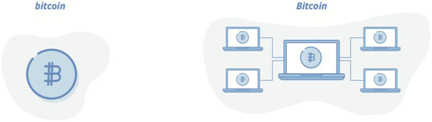
\includegraphics[width=10cm]{imagens/bitcoin-capitulo-1.png}
  \caption*{\textit{\small bitcoin e Bitcoin}}
\end{figure}
  
%\newpage
\section*{De onde veio o Bitcoin?}
%\paragraph{}

O Bitcoin foi inventado por uma pessoa ou grupo de pessoas, conhecido pelo pseudônimo de Satoshi Nakamoto, por volta de 2008. Ninguém sabe a identidade dessa(s) pessoa(s) e, pelo que sabemos, sumiram, não se houve falar dele(s) há anos.

Em 11 de fevereiro de 2009, Satoshi revelou o primeiro protótipo do Bitcoin em um fórum online para os cypherpunks, pessoas que trabalham com tecnologia de criptografia e se preocupam com a privacidade individual.
Embora esse não seja o primeiro anúncio do Bitcoin, contém um bom sumário das motivações de Satoshi, o usaremos para fundamentar nossa discussão.

Extraí as partes relevantes abaixo. Na próxima seção, explicaremos algumas dessas declarações e as motivações de Satoshi para a invenção do Bitcoin e quais problemas ele buscava solucionar.

\begin{quotation}\begin{samepage}
\enquote{\textit{
Desenvolvi um novo sistema de e-cash P2P de código aberto chamado Bitcoin. É totalmente descentralizado, sem servidor central ou partes confiáveis, porque tudo é baseado em criptografia ao invés da confiança. [\ldots]}

\textit{A raiz do problema com a moeda convencional é toda a confiança necessária para fazê-la funcionar. O banco central deve ser confiável para não depreciar a moeda, mas a história das moedas fiduciárias está cheia de violações dessa confiança. Os bancos devem ser confiáveis para manter nosso dinheiro e transferi-lo eletronicamente, mas eles o emprestam em ondas de bolhas de crédito ficando apenas com uma fração na reserva. Temos que confiar neles à nossa privacidade, confiar que não irão permitir que ladrões de identidade drenem nossas contas. Seus enormes custos indiretos tornam os micro pagamentos impossíveis.}

\textit{Na geração passada, os sistemas de compartilhamento de tempo multiusuário tinham um problema semelhante. Antes da criptografia forte, os usuários tinham que confiar na proteção por senha para proteger seus arquivos[\ldots]}

\textit{Então, a criptografia forte tornou-se disponível para as massas e a confiança não era mais necessária. Os dados podiam ser protegidos de uma forma fisicamente impossível para outras pessoas acessarem, não importa por que razão, não importa quão boa seja a desculpa, não importa o quê seja criptografado.}
 
\textit{É hora de termos o mesmo no nosso dinheiro. Com a moeda eletrônica baseada em prova criptográfica, sem a necessidade de confiar em um intermediário, o dinheiro pode ser seguro e as transações com o mínimo de esforço.[\ldots]}
 
\textit{A solução do Bitcoin é usar uma rede ponto a ponto para verificar se há gastos duplos. Em suma, a rede funciona como um servidor de carimbo de data/hora distribuído, carimbando a primeira transação a gastar uma moeda. Ele tira proveito da natureza da informação ser fácil de ser espalhada, mas difícil de ser reprimida. Para obter detalhes sobre seu funcionamento, consulte o design desta solução no artigo disponibilizado em
\newline \textcolor{red}{http://www.bitcoin.org/bitcoin.pdf}}}
\begin{flushright} -- Satoshi Nakamoto
\end{flushright}\end{samepage}\end{quotation}

Quando o Bitcoin foi lançado, apenas algumas pessoas o utilizavam e executavam seu sistema em seus computadores (chamados de \textit{nodes}) para alimentar a rede Bitcoin. A maioria das pessoas na época achou que era uma piada ou que o sistema revelaria sérias falhas no projeto, que o tornaria impraticável.

Com o tempo, mais pessoas se juntaram à rede, usando seus computadores para adicionar segurança à ela e reforçando seu valor, trocando outras moedas pelo Bitcoin ou aceitando-a por bens e serviços. Hoje, dez anos depois, é usado por milhões de pessoas com dezenas a centenas de milhares de nodes executando o software gratuito do Bitcoin, que é desenvolvido por centenas de voluntários e empresas em todo o mundo.

O Bitcoin não foi uma invenção criada do nada. Em seu artigo, Satoshi citou várias tentativas importantes de implementar sistemas semelhantes, incluindo o b-money de Wei Dai e o Hashcash de Adam Back. A invenção do Bitcoin apoiou-se nos ombros de gigantes e, no entanto, foi profunda em sua simplicidade ao criar o primeiro sistema verdadeiramente descentralizado - isto é, que não está sob controle de uma pessoa - para emitir e transferir dinheiro digital.

%\newpage
\section*{O Bitcoin resolve quais problemas?}
%\paragraph{}
 
Vamos detalhar algumas das postagens do Satoshi. Ao longo do livro, abordaremos como esses conceitos são realmente implementados. Não é importante que você entenda imediatamente todos os conceitos difíceis desta seção, mas você vai querer ver quais eram os objetivos do Satoshi, para que possamos almejá-los à medida que avançamos no exercício de \textit{Inventar o Bitcoin}.


\paragraph{}
\textit{Desenvolvi um novo sistema de e-cash P2P de código aberto}
\paragraph{}

O P2P significa ponto a ponto (\textit{peer-to-peer}, no inglês) e indica um sistema onde uma pessoa pode interagir com outra sem intermediários, como sendo pares iguais. Você deve se lembrar das tecnologias de compartilhamento de arquivos P2P, como Napster, Kazaa e BitTorrent, que permitiam que as pessoas compartilhassem música sem baixá-las de um site. O Satoshi projetou o Bitcoin para permitir que as pessoas troquem \textit{e-cash}, dinheiro eletrônico, sem passar por um intermediário da mesma maneira.

O software é de \textit{código aberto}, o que significa que qualquer pessoa pode ver como funciona e contribuir para o projeto. Isso é importante porque elimina a exigência de confiança no próprio Satoshi. Não precisamos acreditar em nada que o Satoshi escreveu em sua postagem sobre como o software funciona. Podemos olhar o código e verificar como ele funciona nós mesmos. Melhor ainda, se não gostarmos de algo, podemos mudar.

\paragraph{}
\textit{É totalmente descentralizado, sem servidor central ou partes confiáveis[\ldots]}
\paragraph{}

Satoshi menciona que o sistema é \textit{descentralizado} para diferenciá-lo de sistemas que possuem controle central. As tentativas anteriores de criar um dinheiro digital como o DigiCash de David Chaum de 1989, eram apoiadas por um \textit{servidor central}, um computador ou conjunto de computadores que era responsável pela emissão e verificação de pagamento, administrado por uma empresa.

Esses esquemas de emissão de dinheiro privado, controlados por uma entidade central, estavam fadados ao fracasso. As pessoas não podem contar com um dinheiro que pode ir embora quando a empresa fecha as portas, é hackeada, sofre uma falha no servidor ou, é fechada pelo governo.

A natureza descentralizada do Bitcoin traz de volta o conceito de dinheiro para o mundo digital: você pode transferi-lo sem falar com ninguém, sem pedir permissão, 24 horas por dia, 365 dias por ano, sem passar por nenhuma autoridade que exige confiança.

\paragraph{}
\textit{\dots tudo é baseado em criptografia ao invés de confiança}
\paragraph{}

A internet e a maioria dos sistemas de computadores modernos são construídos em torno de criptografia, um método de obscurecer informação de tal maneira que apenas o receptor da informação possa decodificar ela.
Como o Bitcoin se livra da exigência de \textit{confiança}? Vamos nos aprofundar neste assunto nos próximos capítulos do livro, mas a ideia básica é que em vez de confiar em alguém que diz "Eu sou Ana" ou "Eu tenho R\$10,00 em minha conta bancária", que significaria acreditar em sua palavra, podemos usar a criptografia matemática para declarar os mesmos fatos de uma forma que seja facilmente verificada pelo destinatário e impossível de ser forjada.
Bitcoin usa criptografia matemática ao longo de todo seu projeto para permitir que participantes possam verificar o comportamento dos mesmos sem confiar em terceiros.
Isso se tornaria a base do sistema do Bitcoin para provar a propriedade dos saldos, bem como fornecer segurança para a rede.

\paragraph{}
\textit{Temos que confiar [nos bancos] nossa privacidade, confiar que não irão permitir que ladrões de identidade drenem nossas contas.}
\paragraph{}

Ao contrário de usar sua conta bancária, sistema de pagamento digital ou cartão de crédito, o Bitcoin permite que duas partes façam transações sem fornecer nenhuma informação de identificação pessoal.

Os repositórios centralizados de dados de consumidores armazenados em bancos, empresas de cartão de crédito, processadores de pagamentos e governos são chamarizes gigantescos para os hackers. Quase que para provar o ponto de Satoshi, a Equifax, foi imensamente comprometida em 2017, quando hackers conseguiram vazar as identidades e dados financeiros de mais de 140 milhões de pessoas.

O Bitcoin separa as transações financeiras das identidades do mundo real. Afinal, quando damos dinheiro físico a alguém, ela não precisa saber quem somos, nem precisamos nos preocupar se, após essa troca, ela poderá usar algumas informações que demos para roubar o nosso dinheiro. Por que não devemos esperar o mesmo, ou coisa pior, quando usamos o dinheiro digital?

\paragraph{}
\textit{O banco central deve ser confiável para não depreciar a moeda, mas a história das moedas fiduciárias está cheia de violações dessa confiança.}
\paragraph{}

\textit{Fiat}, que em latim, significa “que seja feito”, refere-se à moeda emitida pelo governo e pelo banco central que é decretada como curso legal pelo governo. Historicamente, o dinheiro era escolhido livremente pelos participantes do mercado entre coisas difíceis de serem produzidas, fáceis de serem verificadas e transportadas, como sal, conchas, pedras, prata e ouro.
Toda vez que 'algo' era utilizado como dinheiro havia a tentação de criar mais dele. Se alguém viesse com tecnologia superior para rapidamente criar muitos de 'algo', esse 'algo' perdia valor. Era assim que Colonizadores europeus foram capazes de despir o continente africano de suas riquezas, trocando petecas de vidros, facilmente produzidos, por escravos humanos, dificilmente produzidos. Por isso que ouro foi considerado dinheiro por tanto tempo, era difícil de produzir mais dele rapidamente.

Lentamente, mudamos para uma economia mundial que usava o ouro como dinheiro para uma em que o papel passou a representar uma reivindicação desse metal precioso. Eventualmente, o papel foi totalmente separado de qualquer respaldo físico com o pronunciamento do presidente Nixon, que acabou com a conversibilidade internacional do dólar americano em ouro em 1971. 

O fim deste padrão permitiu que governos e bancos centrais aumentassem a oferta de dinheiro à vontade, diluindo o valor de cada nota em circulação, conhecida como \textit{depreciação}. Embora apoiada pelo governo e impossível de ser resgatável por algo palpável, a moeda puramente fiduciária é o dinheiro que todos conhecemos e usamos no dia a dia, na verdade é um conceito relativamente novo, com menos de um século de vida.

Confiamos que nossos governos não abusarão de suas impressoras, mas não precisamos ir muito longe na história em busca de exemplos de \textit{violação dessa confiança}. Em regimes autocráticos e de planejamento central, em que o governo tem a posse direta da máquina de impressão de dinheiro, como a Venezuela, a moeda perdeu quase todo o seu valor. O bolívar venezuelano passou de 2 bolívar por dólar em 2009 para 250.000 bolívar por dólar em 2019. No momento em que escrevo este livro, a Venezuela está em processo de colapso devido à terrível má gestão de sua economia por seu governo.

Em contraste com a moeda \textit{fiduciária} emitida centralmente, cuja oferta não pode ser prevista, a fim de evitar a \textit{depreciação}, Satoshi projetou um sistema de dinheiro em que a oferta era fixa e emitida a uma taxa previsível e imutável. Haverá apenas 21 milhões de bitcoins, embora cada um possa ser dividido em 100 milhões de unidades, chamadas de satoshis, produzindo um total de 2.1 quadrilhões de satoshis em circulação ate o ano de 2140.

Antes do Bitcoin, os ativos digitais não eram escassos. É fácil copiar um livro digital, arquivo de áudio ou vídeo e enviá-lo a um amigo. As únicas exceções são os ativos digitais controlados por intermediários. Por exemplo, ao alugar um filme no iTunes, você pode assisti-lo em seu dispositivo apenas porque o iTunes controla a entrega do filme e pode interrompê-lo após o término do período de locação. Da mesma forma, seu dinheiro digital é controlado pelo seu banco. É função do banco manter um registro de quanto dinheiro você possui e, se você transferi-lo para outra pessoa, ele pode autorizar ou negar essa transferência.

O Bitcoin é a primeira rede digital que impõe escassez sem intermediários e é o primeiro ativo conhecido pela humanidade cujo fornecimento inalterável e cronograma de emissão são conhecidos com antecedência. Nem mesmo metais preciosos como o ouro têm essa propriedade, uma vez que sempre podemos minerar mais e mais depósitos de ouro a uma taxa imprevisível, se for lucrativo fazê-lo. 
Imagina encontrar um asteroide contendo dez vezes mais ouro que nossas reservas no planeta, o que aconteceria com o preço do ouro dado uma oferta tão abundante.
Bitcoin é imune a tais descobertas e manipulações de demanda. É simplesmente impossível de produzir mais dele.
Veremos como isso é aplicado nos próximos capítulos.

A natureza da dinheiro e o funcionamento do sistema monetário atual são intrínsecos, e neste livro não serão detalhados em profundidade adequada. Caso queiras aprender mais sobre tais fundamentos do dinheiro e como eles se aplicam ao Bitcoin recomendo a leitura do livro \textit{O Padrão Bitcoin} por Saifedean Ammous, como ponto de partida

\paragraph{}
\textit{Os dados podiam ser protegidos de uma forma fisicamente impossível para outras pessoas acessarem, não importando o motivo, quão boa a desculpa, não importando nada[\ldots] É hora de termos o mesmo no nosso dinheiro.}
\paragraph{}

Nossos sistemas atuais de proteção de dinheiro, como quando fazemos um depósito em um banco, dependem de confiar em outra pessoa para fazer o trabalho. Confiar em tal intermediário não requer apenas confiança de que eles não farão algo malicioso ou tolo, e que os hackers não irão roubá-lo, mas também que o governo não confiscará ou congelará os fundos. No entanto, foi demonstrado em todo o mundo, repetidamente, que os governos podem e suprimem o acesso ao dinheiro quando se sentem ameaçados.

Pode parecer bobagem para alguém que mora nos Estados Unidos, ou em outra economia altamente regulamentada, pensar em acordar e ter seu dinheiro confiscado. Ocorreu algo parecido comigo, quando tive meus fundos congelados pelo PayPal simplesmente porque não usava minha conta há meses. Levei mais de uma semana para recuperar o acesso ao “meu” dinheiro. Tenho sorte de morar nos Estados Unidos, um dos poucos países onde pelo menos poderia esperar obter algum alívio legal se o PayPal congelasse meus fundos, e onde tenho a confiança básica de que meu governo e meu banco não roubarão meu dinheiro.

Coisas muito piores aconteceram e estão acontecendo atualmente em países com menos liberdade, como bancos sendo fechados durante colapsos da moeda na Grécia, bancos em Chipre usando depósitos para roubar fundos de seus clientes ou o governo declarando certas notas como sendo sem valor de um dia para o outro, como na Índia, privando as pessoas de sua riqueza, causando corridas em caixas eletrônicos e pessoas morrendo de fome devido à incapacidade de acessar seu capital.

A antiga URSS, onde cresci, tinha uma economia fortemente controlada de modo centralizado, levando a uma escassez massiva de bens. Quando queríamos sair, só podíamos trocar uma quantia limitada de dinheiro por pessoa sob uma taxa de câmbio oficial, controlada pelo governo, que era amplamente desconectada da verdadeira taxa de livre mercado. Efetivamente assim o governou tirou de nós a pouca riqueza que tínhamos através de um controle rígido da economia e movimentos de capitais.

Quando as economias começam a falhar em países autocráticos, elas tendem a implementar controles econômicos rígidos, impedindo as pessoas de sacar seu dinheiro dos bancos, carregá-lo para fora do país ou trocá-lo por moedas que ainda possuem valor, como o dólar americano no livre mercado.
Isso da carta branca ao governo para implementar experimentos econômicos insanos como por exemplo o sistema socialista da URSS.

O Bitcoin fornece um sistema de segurança que não depende da confiança de terceiros para proteger o seu dinheiro. Em vez disso, o Bitcoin torna suas moedas \textit{impossíveis de serem acessadas por outros} sem uma chave especial que só você possui, \textit{não importa por que razão, não importa quão boa seja a desculpa, não importa o quê façam}. Possuindo Bitcoin, você possui a chave para sua liberdade financeira. Bitcoin separa dinheiro do estado.

%O Bitcoin separa o dinheiro do estado e, portanto, fornece um controle sobre autocratas e ditadores, restaurando a liberdade do controle da riqueza e a de transportá-la através das fronteiras sem nenhuma interferência.

\paragraph{}
\textit{A solução do Bitcoin é usar uma rede ponto a ponto para verificar se há gastos duplos[\ldots] como um servidor de carimbo de data/hora distribuído, carimbando a primeira transação para gastar uma moeda.}
\paragraph{}

Uma rede simplesmente se refere à ideia de que vários computadores estão conectados e podem enviar mensagens uns aos outros. A palavra distribuído significa que não há uma entidade central controladora, mas que todos os participantes se coordenam para tornar a rede bem-sucedida.

Em um sistema sem controle central, é importante saber que ninguém está trapaceando. A ideia de \textit{gasto duplo} refere-se à capacidade de gastar o mesmo dinheiro duas vezes. Isso não é um problema com dinheiro físico pois ele sai da sua mão quando o utiliza. Entretanto, transições digitais podem ser copiadas, de maneira similar a músicas ou filmes. Quando movimenta dinheiro através de um banco, o banco garante que o dinheiro não será movido duas vezes. Em um sistema sem entidade central é necessário encontrar uma maneira de impedir o gasto duplo que, na prática, é a mesma coisa que forjar dinheiro.

Satoshi está descrevendo que os participantes da rede Bitcoin trabalham juntos para \textit{marcar o tempo} (colocar em ordem) as transações para que saibamos o que aconteceu primeiro, a fim de evitar que seja possível forjar o dinheiro de maneira digital. Nos próximos capítulos, construiremos esse sistema do zero. Isso nos permitirá detectar falsificações sem depender de nenhum emissor central ou validador de transações.

Bitcoin não foi uma invenção do dia para a noite. Em seu artigo, Satoshi cita diversas tentativas importantes de implementar sistemas similares ao Bitcoin, incluindo o b-money do Wei Dai e o Hashcash do Adam Back. A invenção do Bitcoin foi realizada sobre os ombros de gigantes, mas ninguém até então havia juntado todas as peças corretas, criando o então primeiro sistemas de criação e transferência de dinheiro digital verdadeiramente escasso, sem a necessidade de um controle central. 

A invenção do Bitcoin resolveu uma série de problemas técnicos interessantes relacionados a privacidade, degradação e controle central nos sistemas monetários atuais. Alguns deles são:

\begin{enumerate}
\item Como criar uma rede ponto a ponto na qual qualquer pessoa pode ingressar e participar voluntariamente;
\item Como um grupo de pessoas, que não precisam revelar suas identidades ou confiar umas nas outras, pode manter uma contabilidade compartilhada de valores, mesmo que algumas delas sejam desonestas;
\item Como criar uma verdadeira escassez digital sem um intermediário;
\item Como criar um ativo digital que não seja forjável e seja verificável instantaneamente e resistente a roubo e hacking.
\end{enumerate}

Quando Bitcoin foi lançado apenas um punhado de pessoas utilizavam e rodavam um \textit{node} do software Bitcoin nos seus computadores para alimentar a rede Bitcoin. A grande maioria das pessoas da época pensavam que era uma piada, ou que o sistema iria apresentar serias falhas de projeto que o fariam não funcional. 

Com a passagem do tempo mais pessoas se juntaram a rede, utilizando seus computadores a rede se tornou mais segura e reforçando que rede tinha valor ao trocar outras moedas por ela, ou bens e serviços. Hoje dez anos depois a rede é utilizada por milhões de pessoas com dezenas a centenas de milhares de \textit{nodes} rodando o software gratuito do Bitcoin, que foi desenvolvido por centenas de voluntários e empresas ao redor do mundo.

Vamos descobrir como podemos construir este sistema!
